\documentclass[10pt,letterpaper]{article}

\usepackage[margin=0.75in]{geometry}
\usepackage{tikz}

\begin{document}

  \title{CS 321, Assignment 4}
  \author{Cody Malick\\
  \texttt{malickc@oregonstate.edu}}
  \date{\today}
  \maketitle

\section{}
This is an interesting problem. To get the answer, we need to construct an NFA,
reverse it, then construct a regex statement out of it. So, our initial NFA 
looks like this: \\


\begin{center}
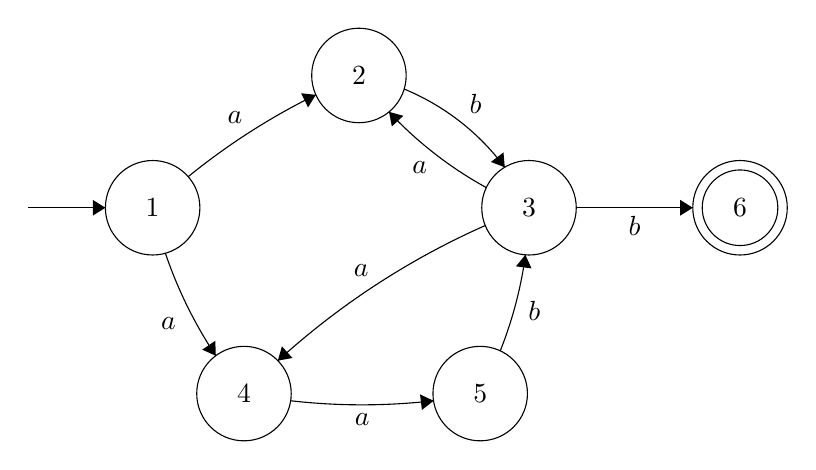
\begin{tikzpicture}[scale=0.2]
\tikzstyle{every node}+=[inner sep=0pt]
\draw [black] (23.6,-23.1) circle (3);
\draw (23.6,-23.1) node {$1$};
\draw [black] (36.7,-14.7) circle (3);
\draw (36.7,-14.7) node {$2$};
\draw [black] (29.4,-34.9) circle (3);
\draw (29.4,-34.9) node {$4$};
\draw [black] (44.4,-34.9) circle (3);
\draw (44.4,-34.9) node {$5$};
\draw [black] (60.9,-23.1) circle (3);
\draw (60.9,-23.1) node {$6$};
\draw [black] (60.9,-23.1) circle (2.4);
\draw [black] (47.5,-23.1) circle (3);
\draw (47.5,-23.1) node {$3$};
\draw [black] (25.858,-21.126) arc (129.14083:116.19689:42.712);
\fill [black] (33.96,-15.93) -- (33.03,-15.83) -- (33.47,-16.73);
\draw (28.82,-17.8) node [above] {$a$};
\draw [black] (41.435,-35.355) arc (-83.43662:-96.56338:39.68);
\fill [black] (41.44,-35.36) -- (40.58,-34.95) -- (40.7,-35.94);
\draw (36.9,-36.12) node [below] {$a$};
\draw [black] (27.609,-32.495) arc (-146.38913:-161.26029:28.018);
\fill [black] (27.61,-32.5) -- (27.58,-31.55) -- (26.75,-32.11);
\draw (25.1,-30.44) node [left] {$a$};
\draw [black] (15.7,-23.1) -- (20.6,-23.1);
\fill [black] (20.6,-23.1) -- (19.8,-22.6) -- (19.8,-23.6);
\draw [black] (39.569,-15.561) arc (67.61395:36.63609:15.158);
\fill [black] (45.96,-20.53) -- (45.88,-19.59) -- (45.08,-20.19);
\draw (44.11,-17.12) node [above] {$b$};
\draw [black] (47.274,-26.09) arc (-7.66574:-21.77358:25.661);
\fill [black] (47.27,-26.09) -- (46.67,-26.82) -- (47.66,-26.95);
\draw (47.43,-29.68) node [right] {$b$};
\draw [black] (50.5,-23.1) -- (57.9,-23.1);
\fill [black] (57.9,-23.1) -- (57.1,-22.6) -- (57.1,-23.6);
\draw (54.2,-23.6) node [below] {$b$};
\draw [black] (44.789,-21.819) arc (-118.77571:-136.97425:24.754);
\fill [black] (38.61,-17.01) -- (38.79,-17.94) -- (39.52,-17.26);
\draw (40.56,-20.16) node [below] {$a$};
\draw [black] (31.555,-32.813) arc (132.33178:113.87159:48.995);
\fill [black] (31.55,-32.81) -- (32.48,-32.64) -- (31.81,-31.9);
\draw (36.85,-27.49) node [above] {$a$};
\end{tikzpicture}
\end{center}

Reverse the NFA: \\

And then tranlate that into a new regex statement:\\
\noindent $b(ba+baa)^*$
\section{}	
\begin{center}
	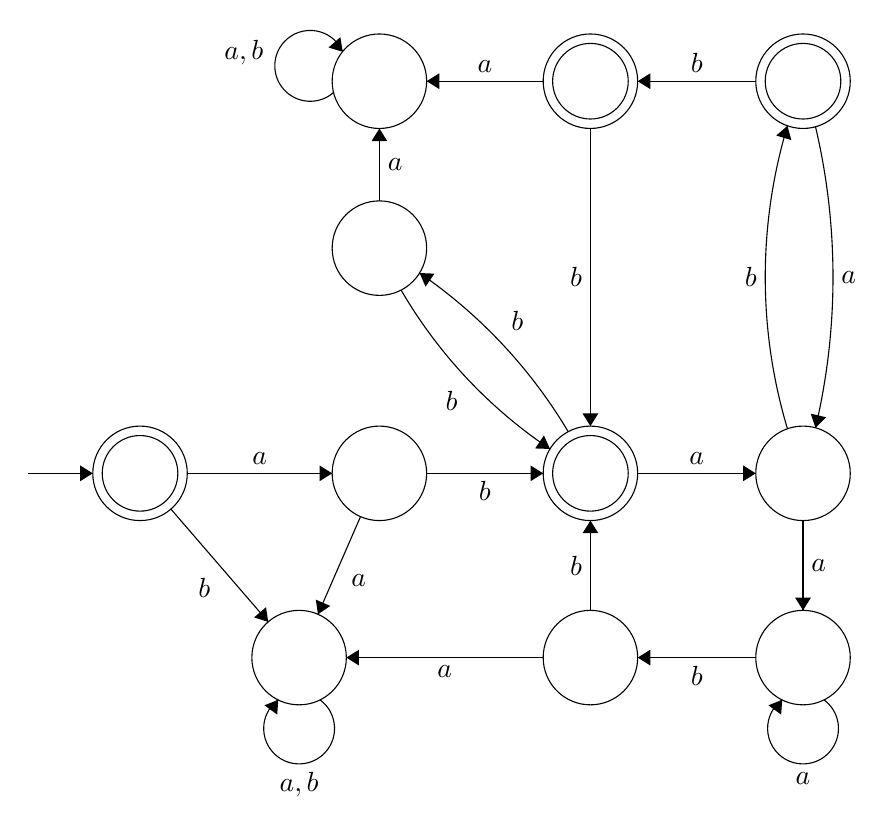
\begin{tikzpicture}[scale=0.2]
		\tikzstyle{every node}+=[inner sep=0pt]
		\draw [black] (10.9,-34.6) circle (3);
		\draw [black] (10.9,-34.6) circle (2.4);
		\draw [black] (26.1,-34.6) circle (3);
		\draw [black] (39.5,-34.6) circle (3);
		\draw [black] (39.5,-34.6) circle (2.4);
		\draw [black] (53,-34.6) circle (3);
		\draw [black] (53,-9.7) circle (3);
		\draw [black] (53,-9.7) circle (2.4);
		\draw [black] (53,-46.3) circle (3);
		\draw [black] (39.5,-46.3) circle (3);
		\draw [black] (21,-46.3) circle (3);
		\draw [black] (39.5,-9.7) circle (3);
		\draw [black] (39.5,-9.7) circle (2.4);
		\draw [black] (26.1,-9.7) circle (3);
		\draw [black] (26.1,-20.3) circle (3);
		\draw [black] (3.8,-34.6) -- (7.9,-34.6);
		\fill [black] (7.9,-34.6) -- (7.1,-34.1) -- (7.1,-35.1);
		\draw [black] (13.9,-34.6) -- (23.1,-34.6);
		\fill [black] (23.1,-34.6) -- (22.3,-34.1) -- (22.3,-35.1);
		\draw (18.5,-34.1) node [above] {$a$};
		\draw [black] (29.1,-34.6) -- (36.5,-34.6);
		\fill [black] (36.5,-34.6) -- (35.7,-34.1) -- (35.7,-35.1);
		\draw (32.8,-35.1) node [below] {$b$};
		\draw [black] (42.5,-34.6) -- (50,-34.6);
		\fill [black] (50,-34.6) -- (49.2,-34.1) -- (49.2,-35.1);
		\draw (46.25,-34.1) node [above] {$a$};
		\draw [black] (52.011,-31.769) arc (-163.30991:-196.69009:33.492);
		\fill [black] (52.01,-12.53) -- (51.3,-13.15) -- (52.26,-13.44);
		\draw (50.1,-22.15) node [left] {$b$};
		\draw [black] (53,-37.6) -- (53,-43.3);
		\fill [black] (53,-43.3) -- (53.5,-42.5) -- (52.5,-42.5);
		\draw (53.5,-40.45) node [right] {$a$};
		\draw [black] (50,-46.3) -- (42.5,-46.3);
		\fill [black] (42.5,-46.3) -- (43.3,-46.8) -- (43.3,-45.8);
		\draw (46.25,-46.8) node [below] {$b$};
		\draw [black] (39.5,-43.3) -- (39.5,-37.6);
		\fill [black] (39.5,-37.6) -- (39,-38.4) -- (40,-38.4);
		\draw (39,-40.45) node [left] {$b$};
		\draw [black] (36.5,-46.3) -- (24,-46.3);
		\fill [black] (24,-46.3) -- (24.8,-46.8) -- (24.8,-45.8);
		\draw (30.25,-46.8) node [below] {$a$};
		\draw [black] (22.323,-48.98) arc (54:-234:2.25);
		\draw (21,-53.55) node [below] {$a,b$};
		\fill [black] (19.68,-48.98) -- (18.8,-49.33) -- (19.61,-49.92);
		\draw [black] (12.86,-36.87) -- (19.04,-44.03);
		\fill [black] (19.04,-44.03) -- (18.9,-43.1) -- (18.14,-43.75);
		\draw (15.4,-41.9) node [left] {$b$};
		\draw [black] (24.9,-37.35) -- (22.2,-43.55);
		\fill [black] (22.2,-43.55) -- (22.98,-43.02) -- (22.06,-42.62);
		\draw (24.28,-41.42) node [right] {$a$};
		\draw [black] (54.323,-48.98) arc (54:-234:2.25);
		\draw (53,-53.55) node [below] {$a$};
		\fill [black] (51.68,-48.98) -- (50.8,-49.33) -- (51.61,-49.92);
		\draw [black] (50,-9.7) -- (42.5,-9.7);
		\fill [black] (42.5,-9.7) -- (43.3,-10.2) -- (43.3,-9.2);
		\draw (46.25,-9.2) node [above] {$b$};
		\draw [black] (36.5,-9.7) -- (29.1,-9.7);
		\fill [black] (29.1,-9.7) -- (29.9,-10.2) -- (29.9,-9.2);
		\draw (32.8,-9.2) node [above] {$a$};
		\draw [black] (23.197,-10.41) arc (311.47119:23.47119:2.25);
		\draw (18.76,-7.86) node [left] {$a,b$};
		\fill [black] (23.77,-7.83) -- (23.62,-6.9) -- (22.87,-7.56);
		\draw [black] (39.5,-12.7) -- (39.5,-31.6);
		\fill [black] (39.5,-31.6) -- (40,-30.8) -- (39,-30.8);
		\draw (39,-22.15) node [left] {$b$};
		\draw [black] (53.793,-12.593) arc (13.2596:-13.2596:41.669);
		\fill [black] (53.79,-31.71) -- (54.46,-31.04) -- (53.49,-30.81);
		\draw (55.4,-22.15) node [right] {$a$};
		\draw [black] (28.649,-21.88) arc (55.52835:30.74977:32.172);
		\fill [black] (28.65,-21.88) -- (29.03,-22.75) -- (29.59,-21.92);
		\draw (34.45,-24.94) node [right] {$b$};
		\draw [black] (36.932,-33.051) arc (-123.88325:-149.83864:30.782);
		\fill [black] (36.93,-33.05) -- (36.55,-32.19) -- (35.99,-33.02);
		\draw (31.1,-30.01) node [left] {$b$};
		\draw [black] (26.1,-17.3) -- (26.1,-12.7);
		\fill [black] (26.1,-12.7) -- (25.6,-13.5) -- (26.6,-13.5);
		\draw (26.6,-15) node [right] {$a$};
	\end{tikzpicture}
\end{center}
\section{}
To show that this DFA has at least 1024 states, we need to prove that having
less that 1024 states rejects a string in $A$, or show that there is a string
not in the language $A$ that the machine accepts. More specifically, we can
show that if machine $M$ has $<1024$ states, then feeding a string with $1024$
characters must prove there is a cycle, showing that it is regular.\\

This can be shown by accounting for every possible combination after the cycle
ends of alphabet $\{a,b\}^*$ leading up to the accepting state. This leaves us
with $2^{10}$ combinations. If we propose that the machine $M$ has less than 1024
states, then we can provide a string of length: number of states + 1, then we
can show there is a string that is rejected by $M$.

Given alphabet $A=\{a,b\}^*$, consider all strings of length 10, $w\in A$. Given
a string of length ten, there are two possible combinations for each position
in the string. Therefore, the total number of possible combinations of strings
are $2^{10}$.

Given that the number of states is less than 1024, then there must be a
combination in the alphabet $A$ that is not accepted. 

\section{}
Step 1:\\
Adversary picks $p$\\
Step 2:\\
I select $w=a^p b^p c^{p-p}$, where $|w|>=p$, and $w \in A$ and $w \in
$ real numbers\\
Step 3:\\
Split into $w=xyz$ where $|xy|=<p$, and $|y|>0$ \\
Step 4:\\
I pick $i=0$, I win if $xy^iz \notin A$\\
Then $xy^0z=xz=a^{p-|y|}c^0 \notin A$ since $|y|>0$\\
I win, A is not regular. 

\end{document}
